\chapter{系统详细设计与实现}

本章节主要旨在介绍Rails消息总线技术开发过程中的关键技术以及关键组件的设计和实现细节,通过对这些组件细节的介绍,描绘出整个系统的实现细节大观。

\section{FileSystemChecker设计}
\subsection{接口设计}
FileSystemChecker类是负责监控特定目录,并且通知特定模块该目录文件系统发生变动的类。该类的定义如图\ref{fig-fuc-class}

\begin{figure}[h]
\centering
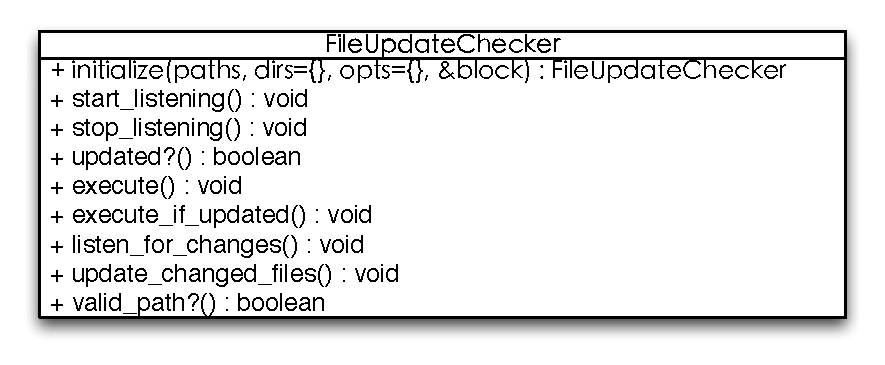
\includegraphics[width=0.6\textwidth]{images/overview/file_update_checker_class.eps}
\caption{FileSystemChecker类图}
\label{fig-fuc-class}
\end{figure}

图\ref{fig-fuc-class}描述了该类所具有的接口,其中initialize接口是该类的构造函数,负责初始化该类的状态。这个接口可接受三个参数,第一个参数是一个数组,该数组包含了所有待监视的目录名。第二个参数是可选参数,它包括了一个哈希表,哈希表是以前一个参数中包含的各个目录名为键,对应的值是一个包含文件拓展名的数组,借此告知FileSystemChecker在对应目录下仅监视该拓展名的文件变动事件。第三个参数则是传入初始化选项,是一个哈希表,它支持如下这些选项:

\begin{itemize}
\item :filter。指明一个正则表达式,使得FileSystemChecker仅仅监视文件名符合该表达式的文件
\item :ignore。指明一个正则表达式,使得FileSystemChecker忽略文件名和该表达式匹配的文件。
\item :notification。指明一个包含Notification名字的数组,当文件变动时FileSystemChecker负责引发这些Notification,这时候如果这个Notification有相应的观察者,则这些观察者将最终收到FileSystemChecker的文件系统变动通知。
\item :recurse。如果该参数为真,则FileSystemChecker会同时监控指明目录的所有子目录。通过对该目录进行深度优先搜索,所有该文件树的文件文件夹新建、修改、删除等事件都能被监控。
\end{itemize}

最后,initialize接口还接受一个Block,这个Block会在每次文件变动被检测到或者execute和execute\_if\_updated被调用是被执行。

start\_listening函数指示FileSystemChecker开进监控文件系统的变动。一旦调用这个方法,程序将会陷入阻塞态,直到其他线程中的代码调用stop\_listening。相应的,stop\_listening负责停止FileSystemChecker对某个文件夹的监控。值得指出的是,一旦FileSystemChecker停止监控后在下一次开始监控时,会将期间所有文件变动通知给消息订阅者。

updated?返回一个布尔值,知名当前是否有文件发生变动,execute将会引发传给构造函数的block的执行,并且会再次检查文件系统是否变动,execute\_if\_updated则是仅仅在有文件变动的前提下执行block。

listen\_for\_changes是监控文件系统的实现函数,这个函数使用深度优先搜索方式搜索文件系统,并且找到文件系统的变动。update\_changed\_files负责实现深度优先搜索。

\subsection{工作流程}
图\ref{fig-fuc-process}展示了FileSystemChecker工作的主要流程:

\begin{figure}[h]
\centering
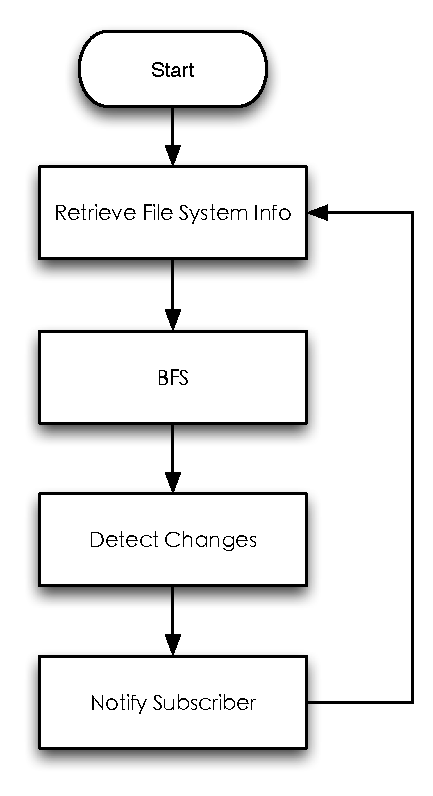
\includegraphics[width=0.4\textwidth]{images/detail/fuc_process.eps}
\caption{FileSystemChecker工作流程图}
\label{fig-fuc-process}
\end{figure}

可以看到,FileSystemChecker在开始监控目录后是以无限循环的形式工作的,在每次循环之前,都会首先获取被监视文件系统的文件信息。实际上,该步骤是给文件系统拍摄快照,用于捕获其当前状态。这之后,FileSystemChecker会对合格树形结构的数据集合进行一个深度优先搜索,通过此实现对所有文件节点的比对。在这之后,FileSystemChecker将当前快照数据同该模块上一次捕获的快照进行比较,借此找出其不同。这些不同则是上次快照捕获到此时文件系统的变化,于是FileSystemChecker便能够即刻发现操作系统文件的变化。当发觉一个或者多个变化后,FileSystemChecker接下来便会通过Notification通知观察者该项变动。值得指出的是,Notification机制是Rails框架内早已存在的一项服务器内部通用消息传送方案,观察者需要首先向某个Notification注册自己,让后方能接收到FileSystemChecker发送的文件变动消息。

\subsection{关键代码}
代码\ref{fuc_core}展示了FileSystemChecker的核心实现:
\begin{lstlisting}[caption={FileSystemChecker核心代码展示}, label=fuc_core]
# Starts listening to changes in the filesystem. This method is
# synchronized until the stop_listening method is called. Once the object
# starts listening, it goes through and checks all files that have been
# changed since the object was created.
#
# If the object was previously stopped, and start_listening is called
# again, then all of the file changes since the last stop was called will
# be pushed to the changed_files queue. The files which were created and
# deleted between the stop and start of the method will be ignored.
def start_listening
  @continue_listening = true
  while @continue_listening
    listen_for_changes
    sleep(0.5)
  end
end

def listen_for_changes
  @semaphore.synchronize do
    @files_alive = []

    paths = initialize_paths(@paths, @dirs)
    directories = handle_paths(paths)
    if @opts[:recurse]
      update_changed_files(directories)
    end

    deleted_files = @file_cache.keys - @files_alive.uniq
    deleted_files.each do |filename|
      @file_cache.delete(filename)
      push_changes(filename, :removed)
    end
  end
end

def update_changed_files(directories)
  new_directory_paths = []

  directories.each do |directory_path|
    expanded_filepaths = Dir.foreach(directory_path)
    .reject { |path| path == ".." || path == "." }  # reject up and self directories on UNIX
    .map { |path| "#{directory_path}/#{path}" }

    new_directory_paths += handle_paths(expanded_filepaths)
  end

  update_changed_files(new_directory_paths) if new_directory_paths.any?
end
\end{lstlisting}

\section{MessageServer设计}
\subsection{接口设计}
MessageServer模块负责实现DRb服务器,和Rinda服务器,使得非服务器进程能够和服务器进程,进而能够向后者委托消息传送任务。其主要类的基本结构如下:

\begin{figure}[h]
\centering
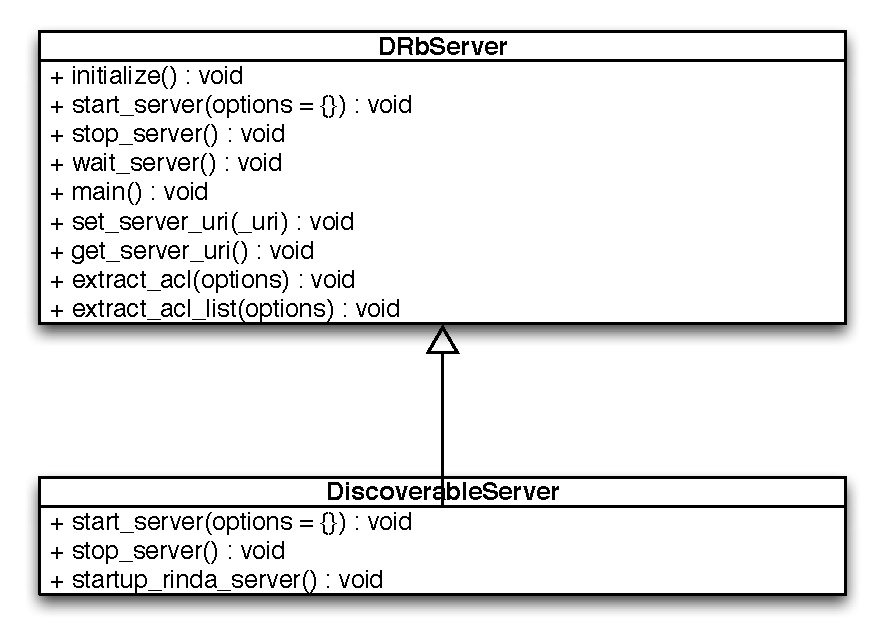
\includegraphics[width=0.6\textwidth]{images/detail/drbserver_class.eps}
\caption{DRbServer及DiscoverableServer类图}
\label{fig-drb-class}
\end{figure}

MessageServer使用DRb技术实现远程过程调用,利用Rinda技术实现服务器的自动发现。DRbServer则是封装了一个用于实现DRb协议的实体类,其接口作用分别如下所示:

initialize是DRbServer类的构造函数,负责构造和舒适化DRbServer类。start\_server负责开启DRb服务器,他的调用将使得DRbServer开始监听本地端口,从而相应远方请求。该接口同时接受一个可选参数,该参数是一个哈希表类型,用acl:作为其键,其值表示一个ACL(Access Control List)列表。该列表的提供主要是基于安全方面的考量,该列表制定了一系列规则,指明了哪些远程主机能够访问本地DRb服务哪些将被拒绝。stop\_server接口则是负责停止DRbServer工作,从而使得本机不再相应远程请求。wait\_server则使执行线程被挂起,等待DRb服务器执行完成,直到其停止执行,方才返回。

main接口主要用作调试,它使得DRbServer拥有一个入口函数,从而使得能够简单的引用改代码从而使得DRb服务器能够执行。set\_server\_uri和get\_server\_uri用于设置和获取DRb服务器的URI。值得指出的是,set\_server\_uri需在DRbServer实际运行之前得以执行,这样DRbServer开启之后便会监听指定的端口,而后者则需要在DRbServer运行之后执行,用于获取当前DRbServer监听的端口。最后,extract\_acl和extract\_acl\_list则与ACL有关,主要用于控制和提取参数中的ACL信息。

DiscoverableServer正如其名所暗示的,负责自动发现服务器。这项机制通过Rinda技术得以实现。由于DiscoverableServer继承于DRbServer,因此大部分的行为和接口语义都和后者一致。除了接口startup_rinda_server,他是DiscoverableServer才有的,负责开启一个Rinda服务器,从而支持服务器自动发现。

上面两个类为MessageServer提供了基础的实现技术,为了使得这两个接口更加便于使用,本技术还提供了一套统一的接口,该接口可以被DRb服务器、Rinda以及DRb客户端同时使用。其设计类图见图\ref{fig-msg-server-class}

\begin{figure}[h]
\centering
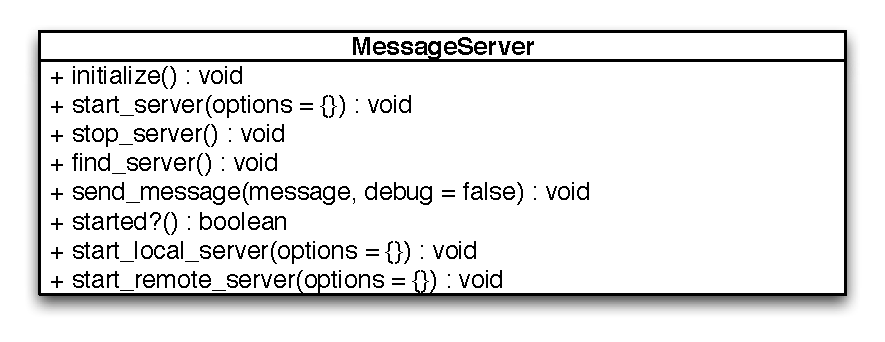
\includegraphics[width=0.6\textwidth]{images/detail/message_bus_class.eps}
\caption{MessageServer类图}
\label{fig-msg-server-class}
\end{figure}



\subsection{工作流程}
\subsection{关键代码}
\section{ActionControler::Live设计}
\subsection{接口设计}
\subsection{工作流程}
\subsection{关键代码}
\section{ActionControler::ServerSentEvents设计}
\subsection{接口设计}
\subsection{工作流程}
\subsection{关键代码}
\section{MessageBus及Instrument Gem设计}
\subsection{接口设计}
\subsection{工作流程}
\subsection{关键代码}










